\documentclass[11pt,a4paper]{article}
\usepackage[margin=2.3cm]{geometry}
\usepackage{graphicx}
\usepackage{booktabs}
\usepackage{xcolor}
\usepackage[colorlinks=true,linkcolor=blue!55!black,urlcolor=blue!55!black]{hyperref}
\usepackage{caption}
\captionsetup{font=small,labelfont=bf}
\graphicspath{{results/}}
\setlength{\parskip}{0.5em}
\setlength{\parindent}{0pt}

\title{\textbf{Section 2, Question 1}\\[0.3em]
       \large Real-Time Log Analytics as a MapReduce Batch Job}
\author{Distributed Systems --- Homework 3}
\date{}

\begin{document}
\maketitle
\vspace{-2.5em}

\section{What the question asks}

Homework~2 Question~7 computed a set of statistics over a server log in a single
sequential program. This question asks for the same statistics, computed as a
\textbf{MapReduce job} so that the work is divided across machines.

The input is $N$ records, each a line of seven numbers:

\begin{center}\small
\texttt{timestamp \quad server\_id \quad endpoint\_id \quad user\_id \quad
status\_code \quad response\_time\_ms \quad bytes\_sent}
\end{center}

The required output is fixed, and includes total, successful and failed request
counts; the average, minimum and maximum response time; total bytes; counts per
HTTP status class; the busiest 60-second interval; and the top $K$ servers and
endpoints by request count. The answer must match the sequential program
\textbf{byte for byte}, whatever the input is divided into.

\section{The idea the solution rests on}

Every quantity above is a \textbf{count, a sum, a minimum or a maximum}. All
four share one property: they can be computed on two halves of the data
independently and combined afterwards, in any order, giving the same answer.
That property --- mergeability --- is what makes the problem expressible as
MapReduce at all.

An average is \emph{not} mergeable, so an average is never stored. The mapper
keeps a sum and a count; the division happens once, in the reducer, when
printing.

Response times are stored as \textbf{whole numbers of millionths of a
millisecond} ($12.5$\,ms becomes $12{,}500{,}000$). Floating-point addition is
not associative, and map tasks finish in a different order on every run, so
decimals could produce a different final digit each time. Integers cannot. One
of the edge-case inputs contains values as small as $10^{-6}$\,ms, which sets
how fine the unit has to be.

\section{What was implemented}

Three standalone C++ programs, each reading standard input and writing standard
output --- which is exactly Hadoop Streaming's contract, so the same binaries
run under Hadoop unchanged.

\begin{center}\small
\begin{tabular}{@{}llr@{}}
\toprule
\textbf{Program} & \textbf{Role} & \textbf{Lines} \\
\midrule
\texttt{mapper.cpp} & reads a split, counts records, emits one line per distinct key & 60 \\
\texttt{combiner.cpp} & merges a mapper's own lines before they travel & 20 \\
\texttt{reducer.cpp} & adds all mappers' lines, computes averages and Top-$K$, prints & 95 \\
\texttt{analytics.h/.cpp} & the shared \texttt{Stats} record and the wire format & 173 \\
\bottomrule
\end{tabular}
\end{center}

\subsection{The pipeline}

\begin{center}\small
\texttt{split} $\rightarrow$ \texttt{mapper} (one per machine) $\rightarrow$
\texttt{sort} (per machine) $\rightarrow$ \texttt{combiner} (per machine)
$\rightarrow$ \texttt{sort} (global) $\rightarrow$ \texttt{reducer} (one)
\end{center}

Four kinds of key travel between the stages: \texttt{G} for the global
counters, \texttt{S:$id$} for one server, \texttt{E:$id$} for one endpoint, and
\texttt{T:$minute$} for one 60-second window. The sort \emph{is} the shuffle ---
no program performs it.

\subsection{Two decisions worth defending}

\textbf{In-mapper combining.} The mapper does not emit a line per record. It
accumulates in memory and emits one line per \emph{distinct key} at the end of
its split. On the ten-million-record input this makes the data crossing the
network $278\times$ smaller than the input ($396$\,MB in, $1.43$\,MB out).
Moving data between machines is the expensive part of MapReduce, so this is the
single most consequential choice in the design.

\textbf{Exactly one reducer.} Top-$K$ requires seeing every server's count
before it can name the largest ten. Two reducers would each produce their own
top ten, and merging those is not the same answer. The single reducer is cheap:
$0.07$\,s against a $16$\,s map stage.

\section{How it was run}

The assignment names Apache Hadoop with YARN. On the RCE cluster that is not
available --- the shared HDFS is read-only for a student account and no
ResourceManager is configured --- and the course confirmed the Hadoop
environment is unavailable, directing students to a Slurm-based script instead.

The benchmark therefore follows the shape of the course's own
\texttt{Mapreduce\_distributed.sh}: \texttt{split} the input, \texttt{srun} a
mapper on each machine, sort locally, combine, sort globally, reduce once.

Measurements use \textbf{one map task per machine}, sweeping 1, 2, 4 and 6
machines. This matters: packing several tasks onto one machine makes them share
a physical core, and the resulting curve describes the scheduler rather than the
program. It is also the allocation shape Assignment~2 used for the MPI version
of this workload, which is what allows the two to be compared.

\section{Results}

Ten million records, median of three runs, every run diffed against the
sequential program.

\begin{center}\small
\begin{tabular}{@{}rrrrrrrr@{}}
\toprule
\textbf{Machines} & \textbf{Total} & \textbf{Map} & \textbf{Sort} &
\textbf{Combine} & \textbf{Gather} & \textbf{Reduce} & \textbf{Speedup} \\
\midrule
1 & 16.940\,s & 16.351 & 0.218 & 0.173 & 0.141 & 0.069 & $1.00\times$ \\
2 & \phantom{0}9.985\,s & \phantom{0}9.478 & 0.160 & 0.124 & 0.152 & 0.071 & $1.70\times$ \\
4 & \phantom{0}5.231\,s & \phantom{0}4.760 & 0.122 & 0.111 & 0.164 & 0.073 & $3.24\times$ \\
6 & \phantom{0}3.637\,s & \phantom{0}3.172 & 0.114 & 0.102 & 0.174 & 0.075 & $\mathbf{4.66\times}$ \\
\bottomrule
\end{tabular}
\end{center}

\textbf{The map stage is the job, and it is CPU-bound.} Mapping accounts for
$16.35$ of $16.94$ seconds --- $97\%$. It would be easy to assume the cost is
reading $396$\,MB from disk, but measuring separately on a compute node,
\texttt{cat} reads the same file in $0.26$\,s while the mapper takes
$13.26$\,s, of which $13.16$\,s is user CPU time. The work is parsing ten
million lines of text, not fetching them. This is why the program scales with
machines at all.

\textbf{The serial tail is real but small.} The global gather, sort and reduce
do not shrink as mappers are added --- they grow slightly, from $0.21$\,s to
$0.25$\,s, because more mappers emit more partial rows for the same keys. That
is $1.2\%$ of the one-machine run but $6.9\%$ of the six-machine run, and it is
what bends the speedup curve away from linear. This is Amdahl's law made
visible.

\textbf{Small inputs should not be distributed.} At $100{,}000$ records, six
machines return only $1.21\times$ over one. Process startup and five pipeline
stages cost more than the work being divided. MapReduce carries a fixed overhead
that is amortised only from roughly a million records upward.

\begin{figure}[htbp]
\centering
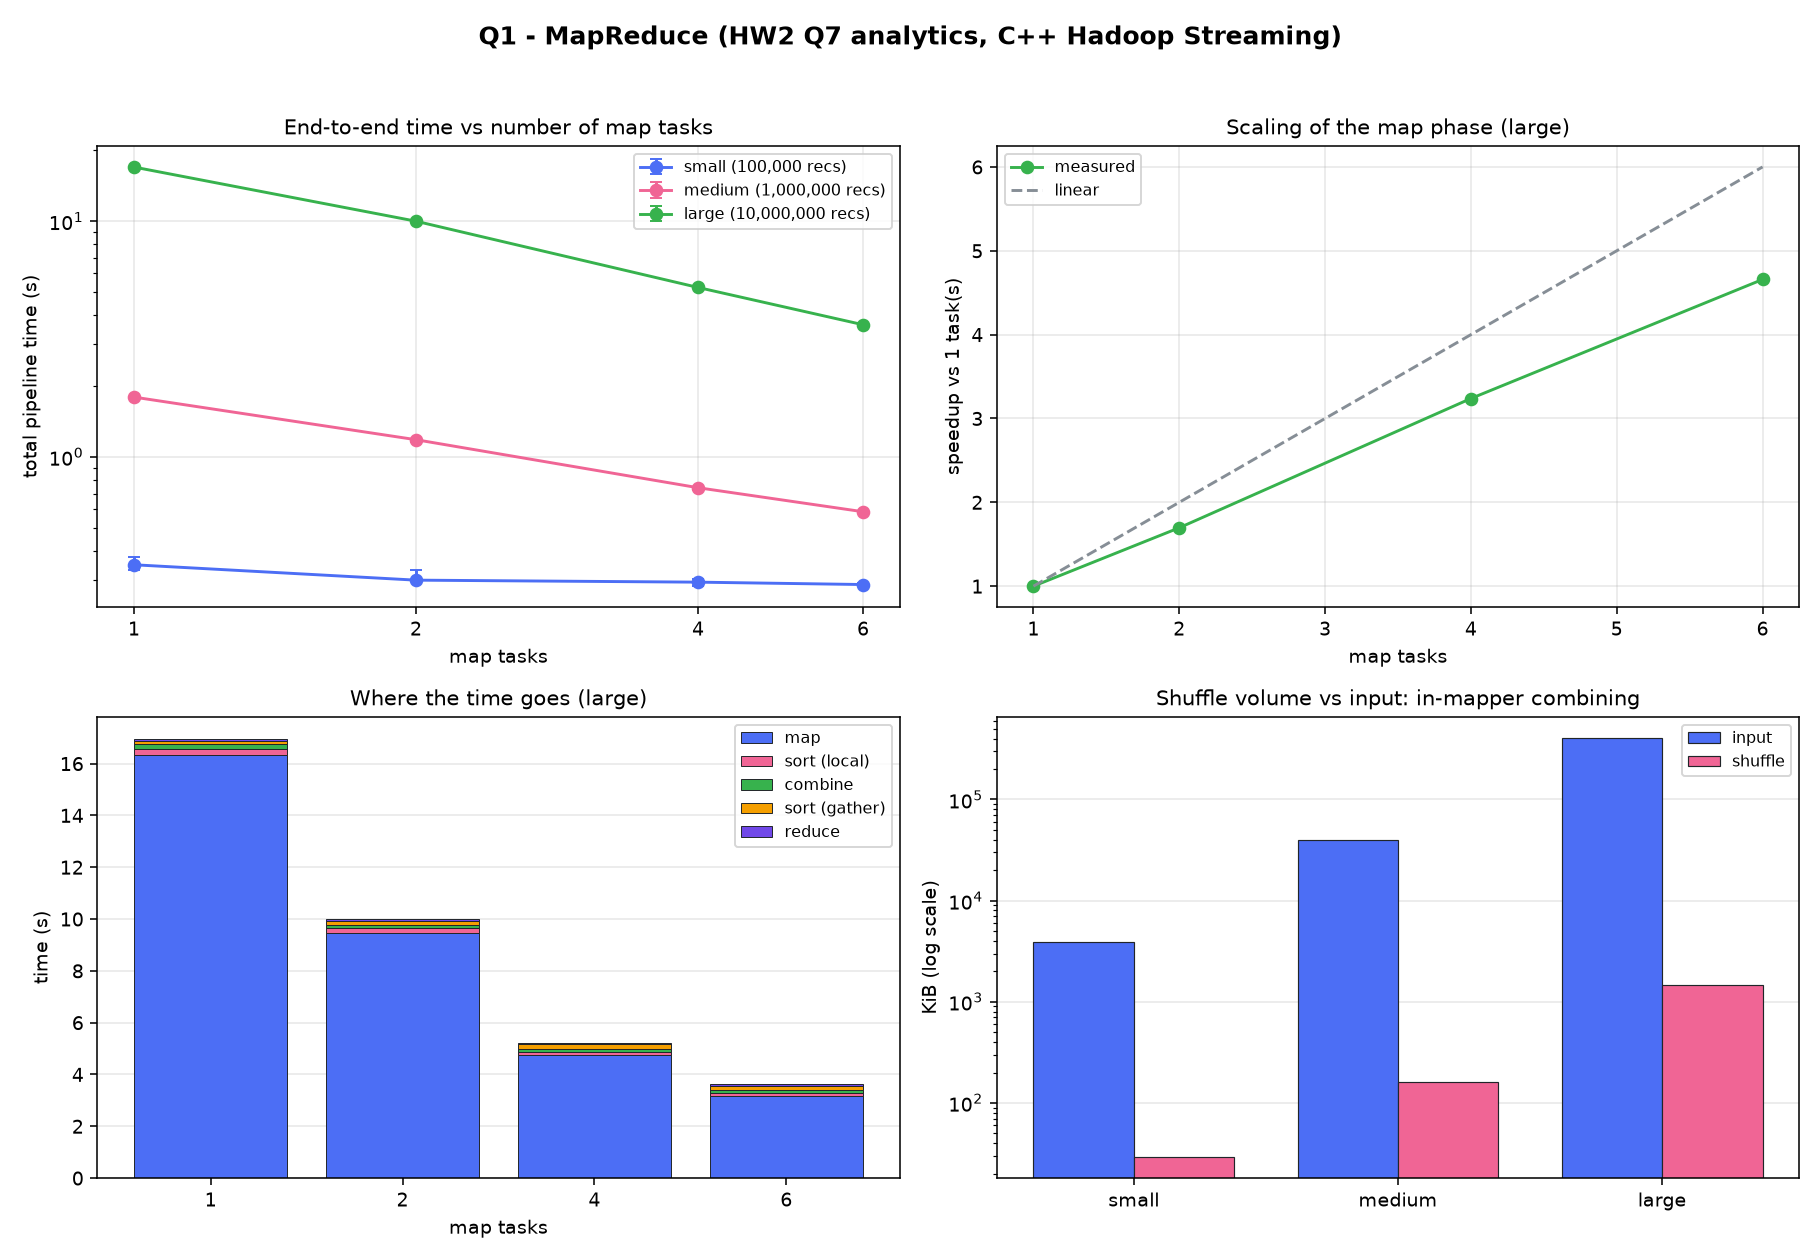
\includegraphics[width=\textwidth]{q1_plots.png}
\caption{End-to-end time against machine count for each dataset; speedup against
the linear ideal; where the time is spent, stacked by stage; and the volume of
intermediate data against the input, showing the effect of in-mapper combining.}
\end{figure}

\subsection{Comparison with MPI}

The same analytics written with MPI, on the same machines, one process each.

\begin{center}\small
\begin{tabular}{@{}rrrr@{}}
\toprule
\textbf{Machines} & \textbf{MPI} & \textbf{MapReduce} & \textbf{MapReduce is} \\
\midrule
1 & 7.441\,s & 16.940\,s & $2.28\times$ slower \\
2 & 4.356\,s & \phantom{0}9.985\,s & $2.29\times$ slower \\
4 & 2.401\,s & \phantom{0}5.231\,s & $2.18\times$ slower \\
6 & 1.701\,s & \phantom{0}3.637\,s & $2.14\times$ slower \\
\bottomrule
\end{tabular}
\end{center}

MPI is faster at every size, which is the expected outcome: it performs no
shuffle, no sort, no serialisation to text and no process creation per stage. It
holds state in memory and reduces once at the end.

Two things are more interesting than the headline. First, \textbf{the gap
narrows} as machines are added, $2.28\times$ down to $2.14\times$. Second,
MapReduce scales slightly \emph{better} over this range --- $4.66\times$ against
MPI's $4.37\times$ --- because its larger constant costs are precisely the part
that parallelises, whereas MPI's closing reduction does not.

\begin{figure}[htbp]
\centering
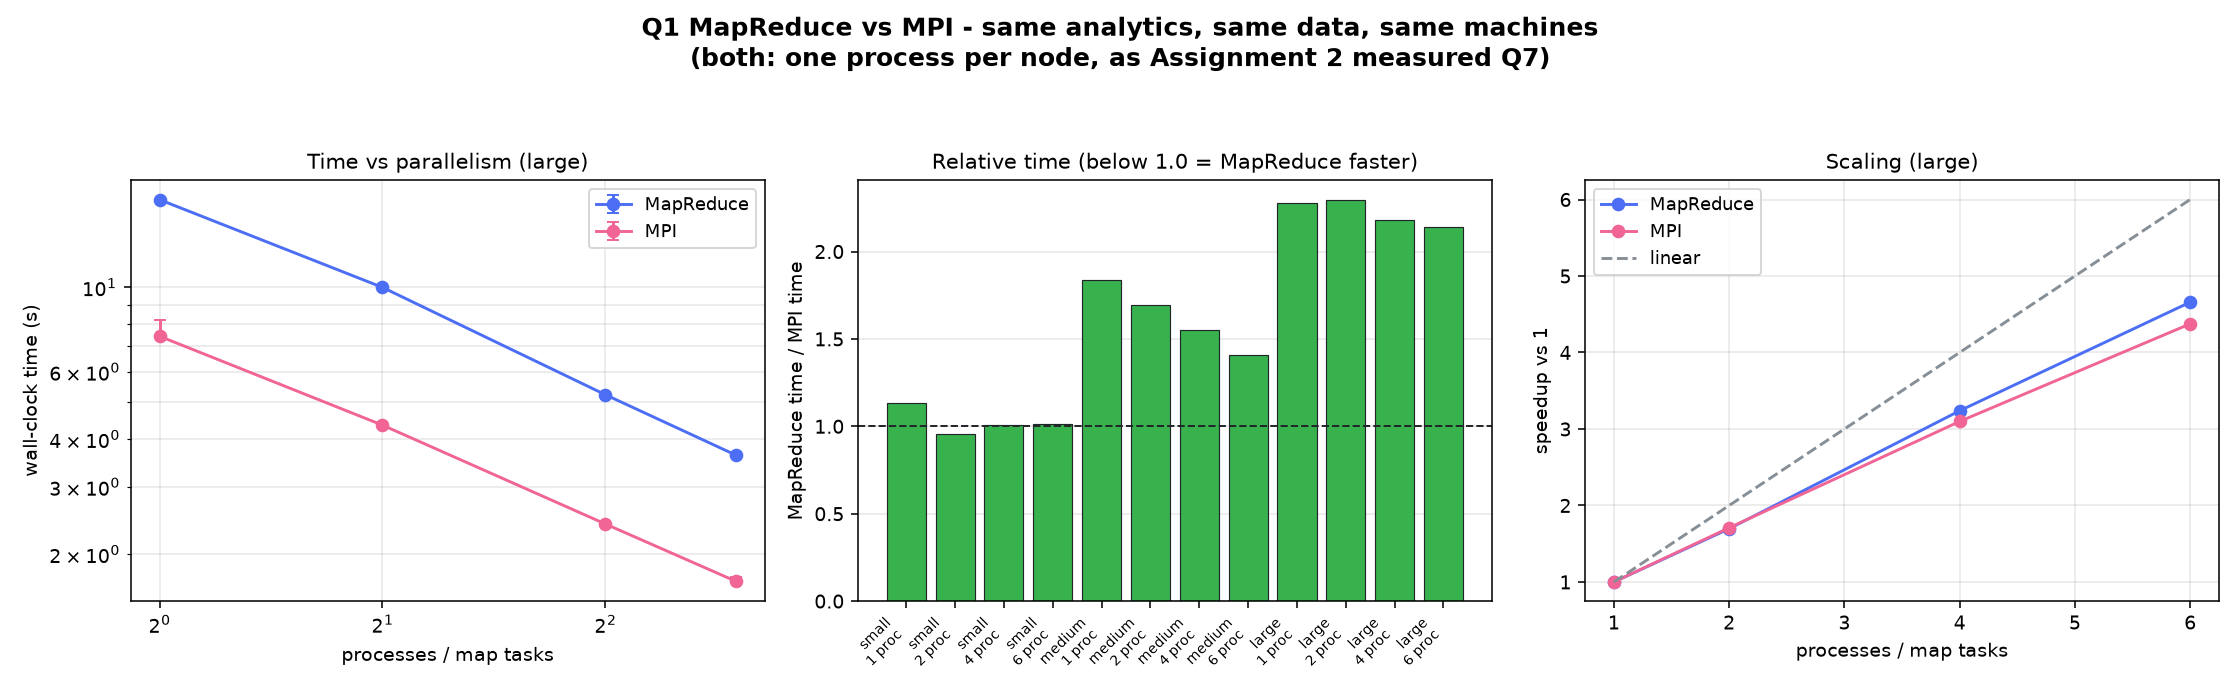
\includegraphics[width=\textwidth]{q1_vs_mpi.png}
\caption{MapReduce against MPI on identical work and identical machines. Left:
wall-clock time against machine count. Centre: the ratio, above $1.0$
throughout but falling. Right: both scale comparably, so the difference lies in
the constant factor rather than in the decomposition.}
\end{figure}

\subsection{Where the constant factor comes from}

The two programs differ in how they represent state, not in their parallel
structure.

\begin{center}\small
\begin{tabular}{@{}llrr@{}}
\toprule
\textbf{Program} & \textbf{State} & \textbf{Peak memory} & \textbf{Time} \\
\midrule
HW2 sequential & two passes, all records buffered, dense arrays & 395\,MB & \phantom{0}4.65\,s \\
MPI, one rank & the same, with a byte-range split & 403\,MB & \phantom{0}6.31\,s \\
Mapper (this work) & one streaming pass, sparse maps & \textbf{10.1\,MB} & 13.00\,s \\
\bottomrule
\end{tabular}
\end{center}

The Homework~2 design pre-scans the input to learn the range of server and
endpoint identifiers, allocates dense arrays, and then indexes them directly:
one array subscript per record, which is as fast as this computation can be. The
price is holding all ten million records in memory first.

A mapper cannot do this. It sees only its own split and therefore cannot know
the global identifier ranges in advance, so it counts in a single streaming pass
into sparse associative containers, discarding each record once counted. The
price is a tree lookup per record instead of an array subscript.

The result is a \textbf{$39\times$ reduction in memory for roughly $2.8\times$
the time}. This is not a defect in either program but a genuine engineering
trade --- and the memory property is exactly what permits the decomposition in
the first place. A design needing $395$\,MB per task and a prior pass over the
whole input cannot be split across mappers that each see a fraction of the data.

\section{Correctness}

Thirty-four checks, all passing, each diffed byte-for-byte against the
unmodified Homework~2 sequential program kept in \texttt{reference/}. They cover
the assignment's worked example, five edge cases (empty input, a single record,
ties in Top-$K$, $K=0$, and response times of $10^{-6}$\,ms), and the same input
divided 1, 2, 4 and 8 ways --- because a correct decomposition must give an
identical answer however the input is divided. All $36$ runs of the performance
sweep matched as well.

\section{Conclusions}

The workload suits MapReduce because every quantity it computes is mergeable,
and the in-mapper combining that mergeability permits reduces network traffic by
$278\times$. The implementation scales $4.66\times$ on six machines, limited by
a small but growing serial tail rather than by the map stage.

It is about $2.2\times$ slower than an equivalent MPI program, and the reason is
identifiable and defensible: sparse streaming state instead of dense buffered
state, which costs time and saves $39\times$ the memory. That trade is not
incidental to MapReduce --- it is what makes a job splittable across machines
that never see the whole input.
\end{document}
